\chapter{Teoria del simplesso}
\section{Terminologia}

\subsection{Equazione della frontiera di un vincolo}
\begin{minipage}{0.45\textwidth}
    È intuitivo pensare che le soluzioni ottimali di un problema di programmazione lineare giacciano sulla frontiera della regione ammissibile, ed infatti ciò corrisponde al vero.
    
    A causa del fatto che la frontiera è un concetto geometrico, la prima definizione che forniamo mira a chiarire come identificare algebricamente la frontiera per una data regione ammissibile.
    
    \textbf{L'equazione della frontiera di un vincolo} viene ricavata con le seguenti sostituzioni:
    \begin{itemize}
        \item $\leq \to =$
        \item $\geq \to =$
    \end{itemize}
\end{minipage}
\hfil
\begin{minipage}{0.45\textwidth}
    \begin{center}
        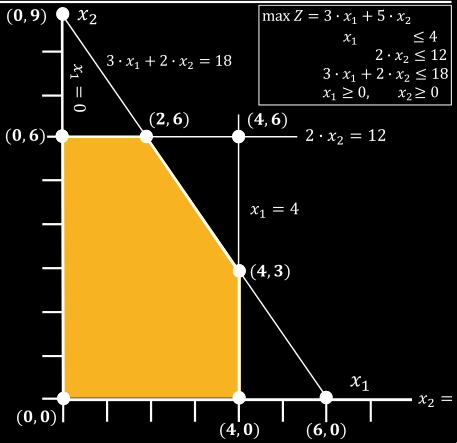
\includegraphics[scale=0.5]{Immagini/equazione della frontiera di un vincolo.png}
    \end{center}
\end{minipage}

\subsection{Equazione della frontiera di un vincolo funzionale}
\begin{minipage}{0.45\textwidth}
    \textbf{L'equazione della frontiera di un vincolo funzionale} è:
    {
        \large
        $$
        a_{i1} \cdot x_1 + a_{i2} \cdot x_2 + \dots + a_{in} \cdot x_n = b_i
        $$
    }
    mentre per un \textbf{vincolo di non negatività abbiamo}:
    {
        \large
        $$
        x_j=0
        $$
    }

    Ogni equazione definisce una \textbf{figura geometrica "piatta"}, che prende il nome di \textbf{IPERPIANO} nello \textbf{spazio n-dimensionale}, l'analogo di una retta nello spazio 2-dimensionale e di un piano nello spazio 3-dimensionale

    \begin{itemize}
        \item Quando il vincolo è di $\leq$ o di $\geq$, l'iperpiano separa i punti che verificano il vincolo da quelli che lo violano
        \item Quando il vincolo è di $=$, solo i punti che giacciono sull'iperpiano verificano il vincolo.
    \end{itemize}
\end{minipage}
\hfil
\begin{minipage}{0.45\textwidth}
    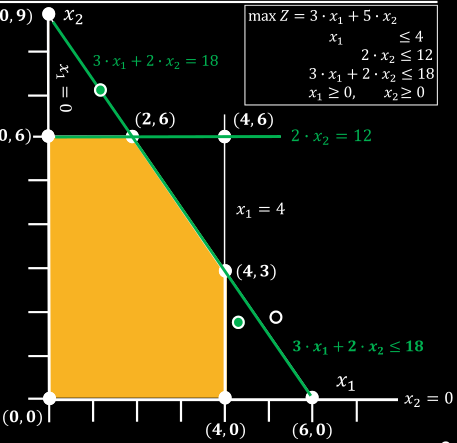
\includegraphics[scale=0.5]{Immagini/equazione della frontiera di un vincolo funzionale.png}
\end{minipage}

\subsection{Frontiera della regione ammissibile}
\begin{minipage}{0.45\textwidth}
    \begin{itemize}
        \item 5 vincoli, 3 funzionali e 2 di non negatività
        \item 5 equazioni di frontiera
        \item $n=2$, gli iperpiani corrispondenti alle equazioni di frontiera sono 5 rette
    \end{itemize}

    La \textbf{frontiera della regione ammissibile} contiene solo quelle soluzioni ammissibili che soddisfano una o più \textbf{equazioni di frontiera}

    Geometricamente, ogni punto sulla frontiera della regione ammissibile giace su uno o più iperpiani definiti dalle rispettive equazioni di frontiera.

    La frontiera corrisponde ai 5 "segmenti spessi" nella figura a destra
\end{minipage}
\hfil
\begin{minipage}{0.45\textwidth}
    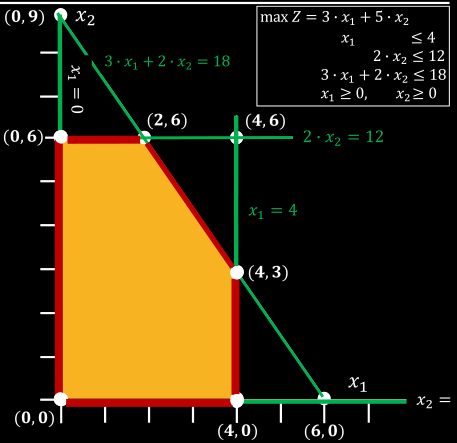
\includegraphics[scale=0.5]{Immagini/Frontiera della regione ammissibile.png}
\end{minipage}

\subsection{Vertice ammissibile}
\begin{minipage}{0.45\textwidth}
    Un \textbf{vertice ammissibile} è una soluzione ammissibile che non giace su un segmento che connette altre 2 soluzioni ammissibili.

    Una soluzione che giace su un segmento che collega due altre soluzioni ammissibili non è un vertice ammissibile.

    \begin{itemize}
        \item $(2,3)$ non è un vertice ammissibile, giace sul segmento che collega $(0,3) \text{ e } (4,3)$
        \item $(0,3)$ non è un vertice ammissibile, giace sul segmento che collega $(0,0) \text{ e } (0,6)$
        \item $(0,0)$ è un vertice ammissibile, non esistono due soluzioni ammissibili tali per cui $(0,0)$ giaccia sul segmento che collega tra loro tali soluzioni ammissibili
    \end{itemize}
\end{minipage}
\hfil
\begin{minipage}{0.45\textwidth}
    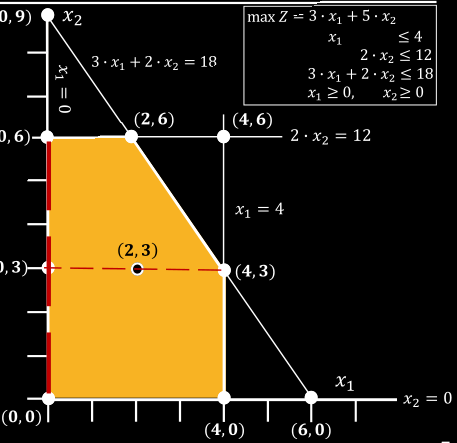
\includegraphics[scale=0.5]{Immagini/Vertice ammissibile_2.png}
\end{minipage}

In ogni problema di programmazione lineare con $n$ variabili di decisione, ogni vertice ammissibile giace all'intersezione di $n$ frontiere di altrettanti vincoli, vale a dire ogni vertice è la soluzione simultanea di un sistema di $n$ equazioni, ognuna rappresentante la frontiera di uno degli $n$ vincoli

\begin{minipage}{0.45\textwidth}
    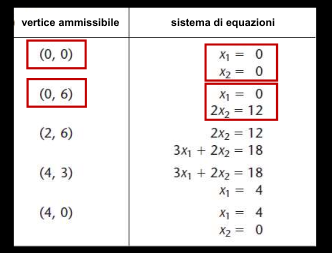
\includegraphics[scale=0.7]{Immagini/Vertice ammissibile_3.png}
\end{minipage}
\hfill
\begin{minipage}{0.45\textwidth}
    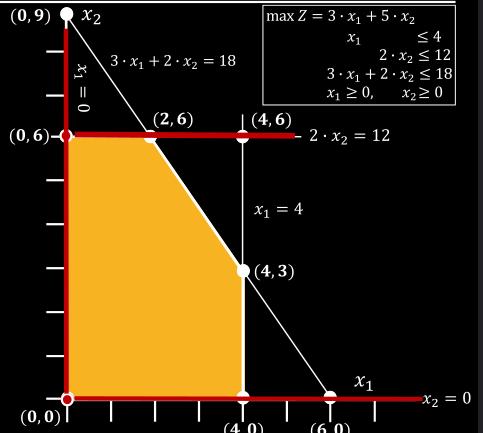
\includegraphics[scale=0.45]{Immagini/vertice ammissible_4.png}
\end{minipage}

\subsection{Vertice non ammissibile}
Comunque, questo non significma che ogni insieme di $n$ equazioni di frontiera, comunque scelte tra gli $n+m$ vincoli, determini un vertice ammissibile.

In particolare, la soluzione simultanea di un tale sistema lineare potrebbe violare uno o più degli $m$ vincoli che non sono stati selezionati per definire il sistema lineare, nel quel caso il vertice individuato sarebbe un \textbf{vertice non ammissibile}

\begin{minipage}{0.45\textwidth}
    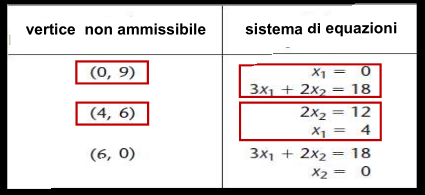
\includegraphics[scale=0.65]{Immagini/vertice non ammissibile_2.png}
\end{minipage}
\hfill
\begin{minipage}{0.45\textwidth}
    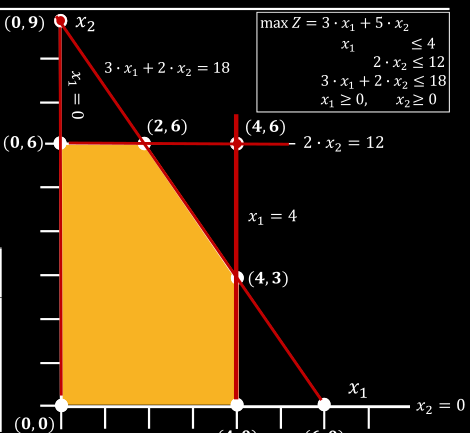
\includegraphics[scale=0.5]{Immagini/vertice non ammissibile_1.png}
\end{minipage}

Inoltre, un sistema di $n$ equazioni potrebbe non ammettere soluzione alcuna.

Questo accade per:
\begin{itemize}
    \item $x_1=0$ e $x_1=4$
    \item $x_2=0$ e $2 \cdot x_2 = 12$
\end{itemize}
sistemi di questo tipo non sono di interesse.

Ultima possibilità (non verificata nel nostro caso) è che esistano \textbf{soluzioni multiple dovute a equazioni ridondanti} il simplesso gestisce per noi queste situazioni

\begin{minipage}{0.45\textwidth}
    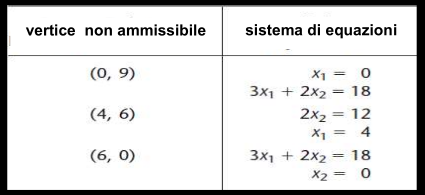
\includegraphics[scale=0.65]{Immagini/vertice non ammissibile_3.png}
\end{minipage}
\hfill
\begin{minipage}{0.45\textwidth}
    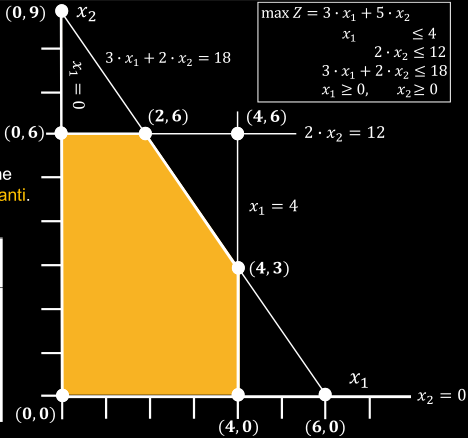
\includegraphics[scale=0.5]{Immagini/vertice non ammissibile_4.png}
\end{minipage}

\begin{minipage}{0.45\textwidth}
    È anche possibile che più di un sistema costituito da $n$ equazioni abbia il medesimo vertice come soluzione
    
    Per esempio se rimpiazziamo il vincolo $x_1 \leq 4$ con il vincolo $x_1 \leq 2$ è possibile constatare come il vertice $(2,6)$ sia ricavabile come soluzione di ogni sistema lineare formato dalle 3 coppie di vincoli
    
    \begin{gather*}
        x_1 \leq 2 \\
        2 \cdot x_2 \leq 12
    \end{gather*}
\end{minipage}
\hfill
\begin{minipage}{0.45\textwidth}
    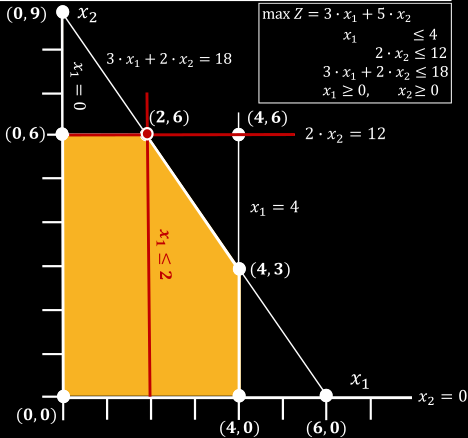
\includegraphics[scale=0.5]{Immagini/vertice non ammissibile 5.png}
\end{minipage}

\section{Vertice ammissibile adiacente}
Quando si ignorano le \textbf{variabili slack e surplus}, abbiamo detto che ogni iterazione dell'algoritmo equivale allo spostamento dal corrente vertice ammissibile a un vertice ammissibile a lui adiacente.

È normale porsi le seguenti domande:
\begin{itemize}
    \item Che \textbf{cammino} segue il metodo del simplesso?
    \item Cose è un \textbf{vertice ammissibile adiacente}
\end{itemize}

La \textbf{frontiera della regione ammissibile} è determinata dagli \uline{spigoli}

\begin{center}
    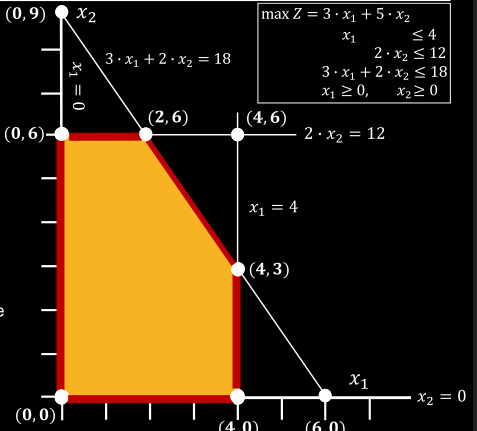
\includegraphics[scale=0.5]{Immagini/vertice ammissibile adiacente_1.png}
\end{center}

\newpage
Da ogni vertice ammissibile emanano due spligoli che conducono ai vertici a lui adiacenti.

Il cammino seguito dal metodo del simplesso nel caso in cui si parla del vertice ammissibile $(0,0)$ è mostrato in foto

Ogni movimento porta ad un vertice ammissibile adiacente, implicando un solo cambio nel sistema di equazioni.

\begin{minipage}{0.45\textwidth}
    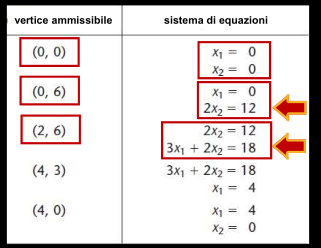
\includegraphics[scale=0.5]{Immagini/vertici ammissibili adiacente_3.png}
\end{minipage}
\hfil
\begin{minipage}{0.45\textwidth}
    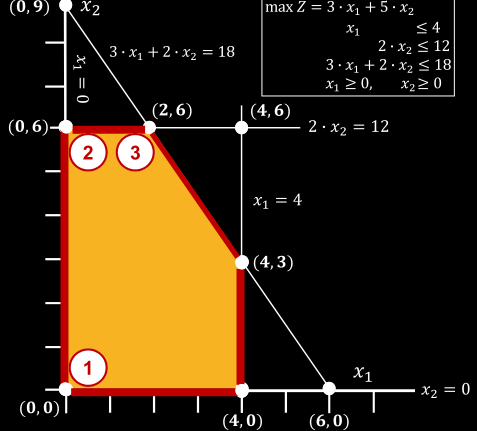
\includegraphics[scale=0.5]{Immagini/vertici ammissibili adiacente_2.png}
\end{minipage}

Nel caso in cui $n=3$ le cose divengono più complesse.

\begin{itemize}
    \item La \textbf{regione ammissibile} non è più un \textbf{poligono} come nel caso di $n=2$ ma un \textbf{poliedro}
    \item Le \textbf{equazioni di frontiera} sono \textbf{piani} e non più \textbf{rette} come nel caso $n=2$
    \item Ogni vertice ammissibile giace all'intersezione di 3 equazioni di frontiera, verificando anche i vincoli restanti.
    \item Le intersezioni che non soddisfano uno o più dei restanti vincoli individuano \textbf{vertini non ammissibili}
\end{itemize}

\begin{center}
    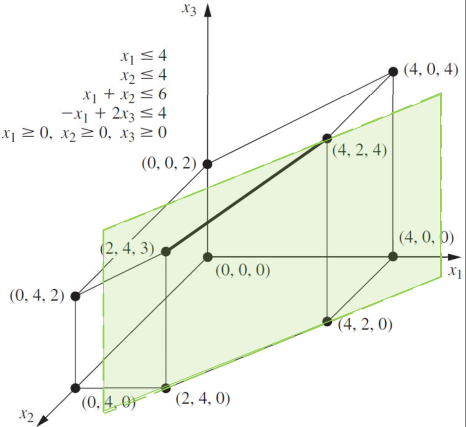
\includegraphics[scale=0.75]{Immagini/poliedro verde.png}
\end{center}

\begin{itemize}
    \item \textbf{Cammino} del metodo del simplesso dal vertice corrente $(2,4,3)$ al vertice adiacente $(4,2,4)$
    \item Il vertice $(2,4,3)$ giace all'intersezione delle seguenti \textbf{equazioni di frontiera}
    \begin{gather*}
        x_2=4 \implies x_1 =4 \\
        x_1 + x_2 = 6 \\
        -x_1 + 2 \cdot x_3 = 4
    \end{gather*}
    
    \item $\mathbf{(2,4,3)}$ e $\mathbf{(4,2,4)}$ sono \textbf{vertici adiacenti}
    \item Per $n=3$ tutti gli \textbf{spigoli della regione ammissibile} sono formati analogamente come intersezione di coppie di equazioni di frontiera 
\end{itemize}

\begin{center}
    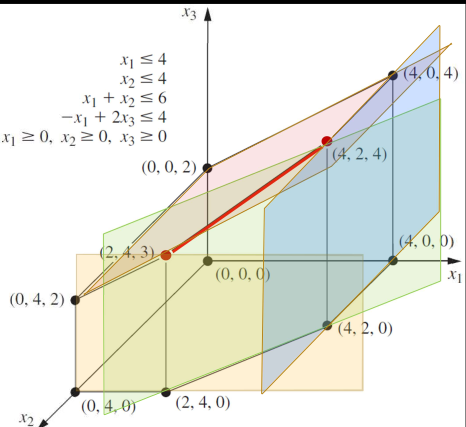
\includegraphics[scale=0.75]{Immagini/poliedro colorato.png}
\end{center}

Se $n>3$, i concetti esposti generalizzano, eccezion fatta per le frontiere dei vincoli che ora sono \textbf{iperpiani} in luogo di \textbf{piani} come nel caso $n=3$.

Dato \uline{un problema di PL con $n$ variabili decisionali e regione ammissibile limitata} avremo che:

\begin{itemize}
    \item Un vertice ammissibile giace all'intersezione di $n$ equazioni di frontiera (e soddisfa anche i restanti vincoli)
    \item Uno spigolo della regione ammissibile è un segmento che giace all'intersezione di $n-1$ equazioni di frontiera, dove ogni vertice estremo giace su un'equazione di frontiera addizionale (tale che gli estremi siano vertici ammissibili)
    \item Due vertici ammissibili sono adiacenti se il segmento che li collega è uno spigolo della regione ammissibile
    \item Da ogni vertice ammissibile emanano $n$ spigoli, ognuno coduce ad uno degli $n$ vertici ammissibili adiacenti
    \item Ogni iterazione del metodo del simplesso si sposta dal corrente vertice ammissibile ad un vertice ammissibile adiacente muovendosi su questi spigoli
\end{itemize}

Passando all'\textbf{interpretazione algebrica} avremo:
\begin{itemize}
    \item L'intersezione delle equazioni di frontiera equivale alla loro risoluzione simultanea in termini del corrispondente sistema lineare
\end{itemize}

Alcune implicazioni diquanto abbiamo appena presentato sono:
\begin{itemize}
    \item Quando il metodo del simplesso \textbf{sceglie la variabile entrante in base}, l'interpretazione geometrica è che il metodo del simplesso stia \textbf{scegliendo uno degli \uline{spigoli} che emanano dal \uline{vertice ammissibile corrente}}
    
    \item \textbf{Aumentare il valore della \uline{variabile entrante in base}}, a partire dal valore zero, e contemporaneamente variare il valore delle restanti variabili di base, \textbf{corrisponde a muoversi lungo lo spigolo scelto}
    
    \item Il valore di una delle variabili di base correnti, in particolare la \textbf{variabile uscente dalla base}, viene \textbf{ridotta fino a raggiungere il valore zero}, il che significa il \textbf{raggiungimento della \uline{frontiera del vincolo}} che si trovano all'altro \textbf{estremo dello \uline{spigolo}} della regione ammissibile
\end{itemize}


\section{Proprietà dei vertici ammissibili}

\subsection{Proprietà 1}
\begin{minipage}{0.45\textwidth}
    \begin{itemize}
        \item [\textbf{a}] Se esiste solo una soluzione ottimale, allora questa è un vertice ammissibile
        \item [\textbf{b}] Se esistono soluzioni ottime multiple (e la regione ammissibile è limitata) allora almeno due di queste soluzioni sono vertici ammissibili tra loro adiacenti
        \item La soluzione ottima $(2,6)$ è un vertice ammissibile
        \item In ogni problema che ammetta una sola soluzione ottimale, è sempre possibile far aumentare il valore della funzione obiettivo fino a che non si raggiunga un vertice (la soluzione ottimale) della regione ammissibile
    \end{itemize}
\end{minipage}
\hfil
\begin{minipage}{0.45\textwidth}
    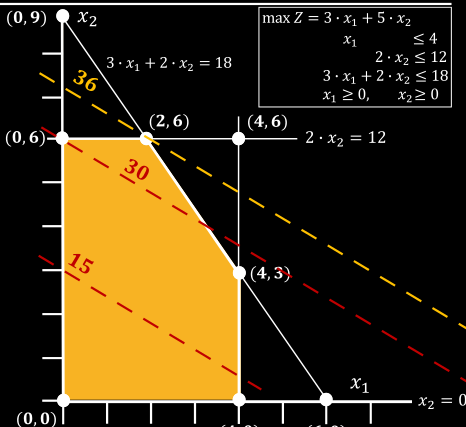
\includegraphics[scale=0.5]{Immagini/Prop1.png}
\end{minipage}

\begin{minipage}{0.45\textwidth}
    Se la funzione obiettivo fosse
    $$
        Z = 3 \cdot x_1 + 2 \cdot x_2
    $$
    
    allora la risoluzione grafica consisterebbe nel far aumentare la funzione obiettivo sino a farla sovrapporre con il segmento (spigolo) che connette il vertice ammissibile $(2,6)$ con il vertice ammissibile $(4,3)$.
    
    Lo stesso accadrebbe nel caso di più variabili di decisione tranne che in quel caso la funzione obiettivo sarebbe associata ad un iperpiano che verebbe fatto aumentare sino a toccare gli spigoli tali da collegare vertici ammissibili adiacenti.
    
    Come conseguenza, \uline{tutte le soluzioni ottimali sono ottenibili come media pesata dei vertici ammissibili ottimali}
\end{minipage}
\hfil
\begin{minipage}{0.45\textwidth}
    \begin{center}
        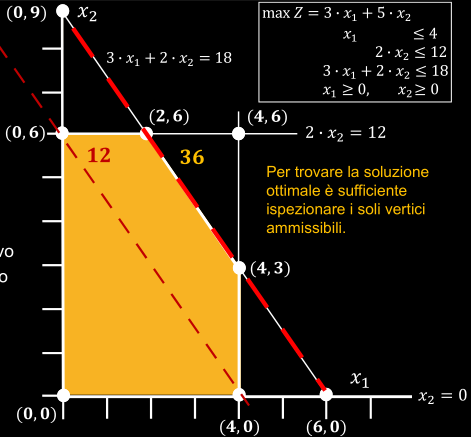
\includegraphics[scale=0.5]{Immagini/Prop1_2.png}
    \end{center}
\end{minipage}

\subsection{Proprietà 2}
\begin{minipage}{0.45\textwidth}
    Esiste un numero finito di vertici ammissibili.

    Ogni vertici ammissibile è soluzioni di un sistema lineare formatoda $n$ equazioni scelte tra $m+n$ vincoli ($n$ vincoli di non negatività ed $m$ vincoli funzionali)

    Il numero di combinazioni di $m+n$ vincoli, presi a gruppi di $n$, è pari a:

    $$
    \frac{(m+n)!}{m!n!}
    $$
    che è un numero finito.

    Questa quantità rappresenta un \uline{limite superiore al numero di vertici ammissibili}
\end{minipage}
\hfill
\begin{minipage}{0.45\textwidth}
    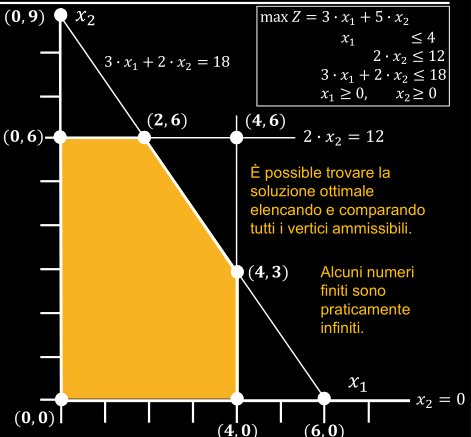
\includegraphics[scale=0.5]{Immagini/Propo2.png}
\end{minipage}

\subsection{Proprietà 3}
\begin{minipage}{0.45\textwidth}
    Se un vertice ammissibile non ammette vertici ammissibili a lui adianceti che coincidono con soluzioni con valore migliore della funzione obiettivo $Z$, allora non esistono soluzioni ottimali migliori di quella che coincide con il vertice ammissibile in esame.

    Pertanto, un tal vertice, in base alla proprietà 1, è garantito coincidere con una soluzione ottimale, e questo semplicemente con assumendo che il problema di PL considerato ammetta almeno una soluzione ottimale, il che è garantito se si assume che il problema di PL abbia soluzione ammissibile e la sua regione ammissibile sia limitata.
\end{minipage}
\hfill
\begin{minipage}{0.45\textwidth}
    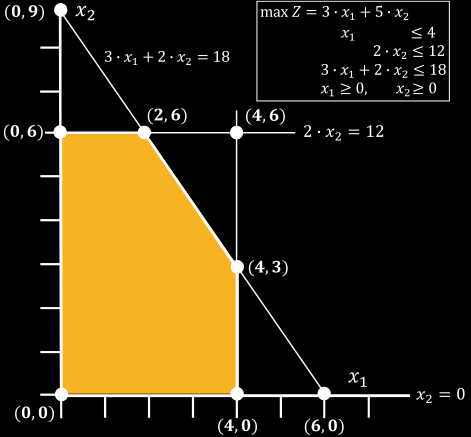
\includegraphics[scale=0.5]{Immagini/Prop3_1.png}
\end{minipage}